\documentclass{article}
\usepackage[utf8]{inputenc}
\usepackage[brazil]{babel}
\usepackage{epsfig}
\usepackage{fancyhdr}
\usepackage{indentfirst} 
\usepackage{titlesec}
\usepackage{amsmath}
\usepackage{amsthm}
\usepackage{listings}
\usepackage{color}


\definecolor{dkgreen}{rgb}{0,0.6,0}
\definecolor{gray}{rgb}{0.5,0.5,0.5}
\definecolor{mauve}{rgb}{0.58,0,0.82}

\lstset{
  language=Python,                
  basicstyle=\footnotesize,           
  numbers=left,                   
  numberstyle=\tiny\color{gray},  
  stepnumber=2,                             
  numbersep=5pt,                  
  backgroundcolor=\color{white},    
  showspaces=false,               
  showstringspaces=false,         
  showtabs=false,                 
  frame=single,                   
  rulecolor=\color{black},        
  tabsize=2,                      
  captionpos=b,                   
  breaklines=true,                
  breakatwhitespace=false,        
  title=\lstname,                               
  keywordstyle=\color{blue},          
  commentstyle=\color{dkgreen},       
  stringstyle=\color{mauve},     
}

\pagestyle{empty}

\headheight 40mm      %
\oddsidemargin 2.0mm  %
\evensidemargin 2.0mm %
\topmargin -40mm      %
\textheight 250mm     %
\textwidth 160mm      %
%
\newcounter{execs}
\setcounter{execs}{0}
\newcommand{\exec}[0]{\addtocounter{execs}{1}\item[\textbf{\arabic{execs}.}]}

\fancypagestyle{first}
{
\pagestyle{fancy}
}
%%%%%%%%%%%%%%%%%%%%%%%%%%%%%%%%%%%%%%%%%%%%%%%%%%%%%%%%
%%%%%%%%%%%%%%%%%%%%%%%%%%%%%%%%%%%%%%%%%%%%%%%%%%%%%%%%
% PLEASE, EDIT THIS!
\fancyhead[LO]{\small $3^a$ Lista \\ 
                DCC008 - Cálculo Numérico  \\
                \textbf{Entrega: 14 de Outubro de 2018} }

\fancyhead[RO]{\small Universidade Federal de Juiz de Fora - UFJF \\ 
                Departamento de Ciência da Computação \\
               \textit{Nome: Thiago de Almeida}\\
               \textit{Nome: Renan Nunes}}


\begin{document}
\thispagestyle{first}

\noindent \textbf{Obs1.:} antes de resolver os exercícios abaixo, teste cada um dos métodos implementados resolvendo sistemas lineares simples de dimensão $3\times 3$ (use um exemplo dos Slides).

\noindent \textbf{Obs2.:} utilize precisão dupla.
\begin{itemize}

\exec Resolva o sistema gerado pela questão 2 da $1^a$ Lista utilizando métodos diretos (Thomas, Gauss, LU e Cholesky) e métodos iterativos (Jacobi e Gauss-Seidel). Para este estudo, considere:

\begin{itemize}
\item Sistemas lineares de diferentes dimensões (ex. 1000, 5000, 10000) a partir do problema resolvido na $1^a$ Lista variando o número de elementos; 
\item A aplicação do critério das linhas para determinar se os métodos iterativos convergem neste caso;
\item O tempo de processamento de cada método, direto ou iterativo, para a resolução do sistema e monte uma tabela;
\item Apresente o critério de parada e a tolerância utilizada para os métodos iterativos;
\item Comente os resultados obtidos.
\end{itemize}


\text O critério de Parada Utilizado nas implementações dos métodos iterativos está no código abaixo. \\
\text Na geração da matriz, foi usado o erro $0,01$.\\
\text E a tolerância dos métodos iterativos usada foi de $0,0001$. 

\subsection*{Python}
\begin{lstlisting}
    def normaMaximo(self, x):
        size = len(x)
        maximo = abs(x[0])   
        
        for i in range(size):
            temp = abs(x[i])        
            if(temp > maximo):
                maximo = temp
                
        return maximo
        
    def distanciaMaximo(self, x1, x2):
        if(len(x1) != len(x2)):
            print("O tamanho dos vetores x1 e x2 precisa ser o mesmo")
            return 0
            
        size = len(x1)
        dist = abs(x1[0] - x2[0])  
        
        for i in range(size):
            temp = abs(x1[i] - x2[i])
            if(temp > dist):
                dist = temp
                
        return dist
            
    def calculaErro(self, x_prox, x_atual):
        return self.distanciaMaximo(x_prox, x_atual) / self.normaMaximo(x_prox)

\end{lstlisting}

\newpage

\text Antes da execução dos métodos iterativos foi feita a verificação do critério das linhas com a implementação abaixo
\subsection*{Python}
\begin{lstlisting}
def checarCriterioDasLinhas(self, M):

        ordem = len(M)

        for i in range(ordem):
            valores = [] 
            div = M[i][i]

            #se algum elemento da diagonal principal for zero
            #a matriz nao satisfaz o criterio das linhas
            if(div == 0):
                return False

            for j in range(ordem):
                if(i != j):
                    valores.append(M[i][j] / div)
                
            #um elemento dividido pelo valor da diagonal principal deu maior ou igual que 1
            #a matriz nao satisfaz o criterio das linhas
            if(max(valores) >= 1):
                return False

        return True
\end{lstlisting}

\text O método que calcula o erro residual da questão 2 também está mostrado abaixo.

\subsection*{Python}
\begin{lstlisting}
    def erroResidual(self, M, X, B):
        size = len(M[0])
        erroRet = []
        for i in range(size):
            valor = 0
            for j in range(size):
                valor += M[i][j] * X[j]

            erroRet.append(abs(valor - B[i]))

        return [erroRet, max(erroRet)]
\end{lstlisting}

\newpage

\text Lembrando que a contagem de passos conta os realizados pelo pivoteamento\\
\text Para uma Matriz 100x100:

\begin{table}[h]
\centering
  \begin{tabular}{l||l|lll}
    $Metodo$ & $Passos$ & $Tempo$ $de$ Execução \\
    \hline
    Thomas (direto) & 9997 & 0:00:00.002952 \\
    
    Gauss (direto) & 328251 & 0:00:00.107486 \\
    
    Gauss com Pivoteamento Parcial & 338052 & 0:00:00.104647 \\
    
    Gauss-Seidel (iterativo) & 4361445 &  0:00:01.201678 \\
    
    LU & 333300  & 0:00:00.324635 \\
    
    Choleski & 24354 & 0:00:00.074590 \\
    
    Jacobi (iterativo) & 46629 & 0:00:00.785732 \\
    \hline
  \end{tabular}
  \caption{Matriz 100x100}
\end{table}


\begin{figure}[!htb]
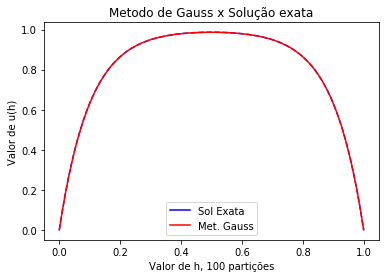
\includegraphics [width=5cm,height=5cm]{G100part.png}
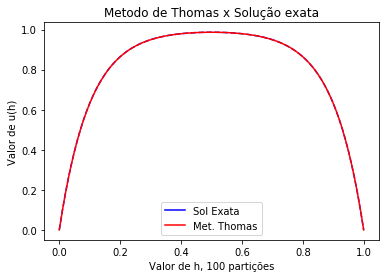
\includegraphics [width=5cm,height=5cm]{T100part}
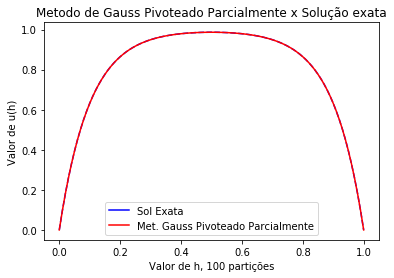
\includegraphics [width=5cm,height=5cm]{GP100part.png}
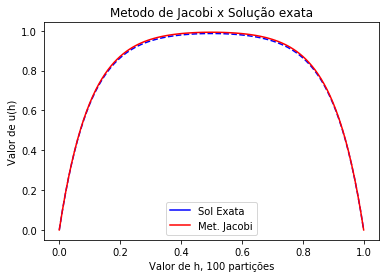
\includegraphics [width=5cm,height=5cm]{J100part.png}
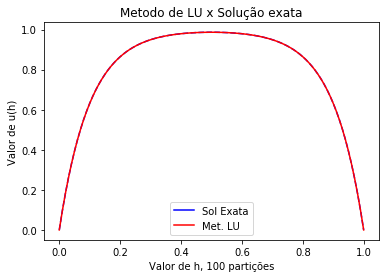
\includegraphics [width=5cm,height=5cm]{LU100part.png}
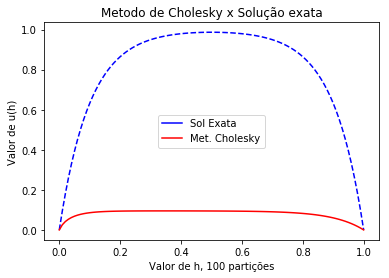
\includegraphics [width=5cm,height=5cm]{Cho100part.png}
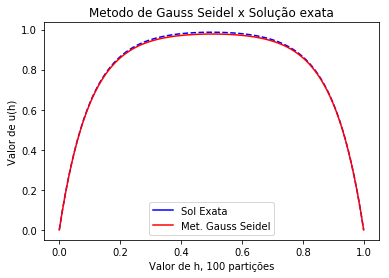
\includegraphics [width=5cm,height=5cm]{GS100part.png}
\end{figure}

\newpage

\text Para uma matriz 1000x1000:

\begin{table}[h]
\centering
  \begin{tabular}{l||l|lll}
    $Metodo$ & $Passos$ & $Tempo$ $de$ Execução \\
    \hline
    Thomas (direto) & 999997  & 0:00:00.235122 \\
    
    Gauss (direto) & 332832501 & 0:01:39.306903\\
    
    Gauss com Pivoteamento Parcial & 333830502 & 0:01:39.587652\\
    
    Gauss-Seidel (iterativo) & 2011970016 &  0:09:22.138811 \\
    
    LU & 333333000 & 0:05:06.996908 \\
    
    Choleski & 2493504  &  0:00:34.001452 \\
    
    Jacobi (iterativo) & 3964032 & 0:06:03.981231  \\
    \hline
  \end{tabular}
  \caption{Matriz 1000x1000}
\end{table}

\begin{figure}[!htb]
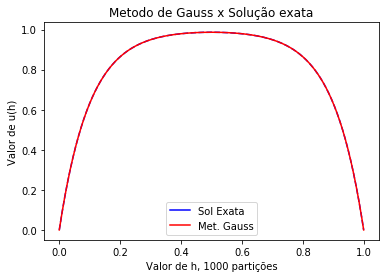
\includegraphics[width=5cm,height=5cm]{G1000part.png}
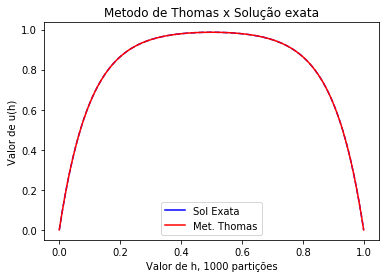
\includegraphics [width=5cm,height=5cm]{T1000part}
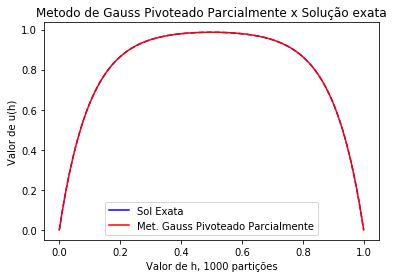
\includegraphics [width=5cm,height=5cm]{GP1000part.png}
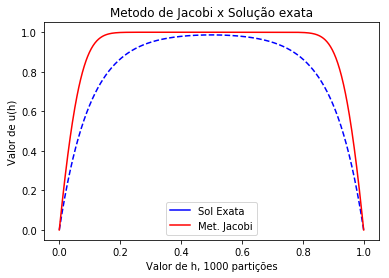
\includegraphics [width=5cm,height=5cm]{J1000part.png}
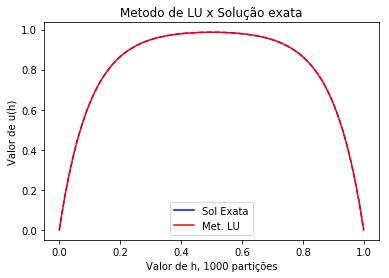
\includegraphics [width=5cm,height=5cm]{LU1000part.png}
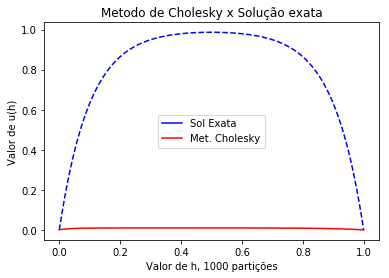
\includegraphics [width=5cm,height=5cm]{Cho1000part.png}
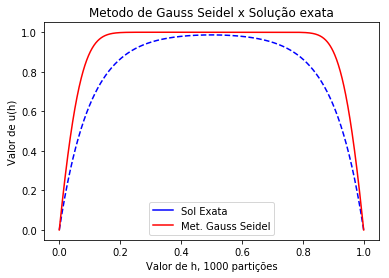
\includegraphics [width=5cm,height=5cm]{GS1000part.png}
\end{figure}


\newpage

\text Para uma matriz 2000x2000:

\begin{table}[h]
\centering
  \begin{tabular}{l||l|lll}
    Metodo & Passos & Tempo de Execução \\
    \hline
    Thomas (direto) & 3999997  & 0:00:01.438566 \\
    
    Gauss (direto) & 2664665001 & 0:12:35.660406 \\
    
    Gauss com Pivoteamento Parcial (direto) & 2668661002 & 0:13:36.051002 \\
    
    Gauss-Seidel (iterativo) & 9270722320  &  0:45:47.694755 \\
    
    LU & 2666666000 & 0:44:35.352543 \\
    
    Choleski & 9987004 & 0:04:44.301479 \\
    
    Jacobi (iterativo) & 9137429 & 0:26:51.788595  \\
    \hline
  \end{tabular}
  \caption{Matriz 2000x2000}
\end{table}


\begin{figure}[!htb]
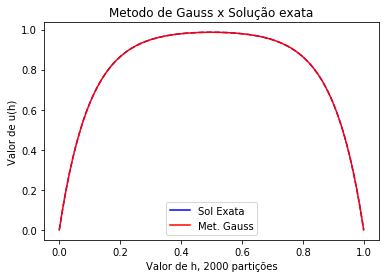
\includegraphics[width=5cm,height=5cm]{G2000part.png}
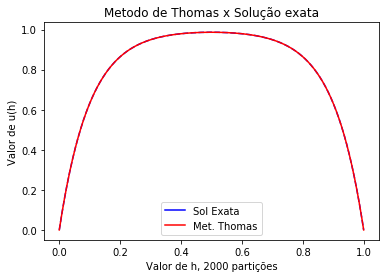
\includegraphics [width=5cm,height=5cm]{T2000part}
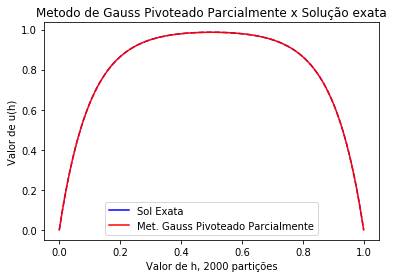
\includegraphics [width=5cm,height=5cm]{GP2000part.png}
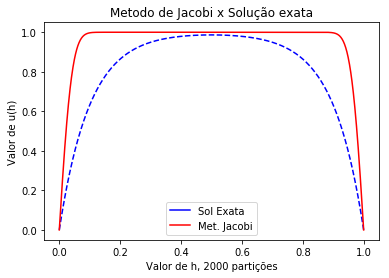
\includegraphics [width=5cm,height=5cm]{J2000part.png}
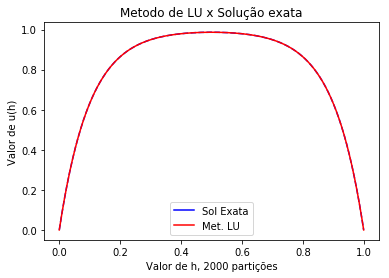
\includegraphics [width=5cm,height=5cm]{LU2000part.png}
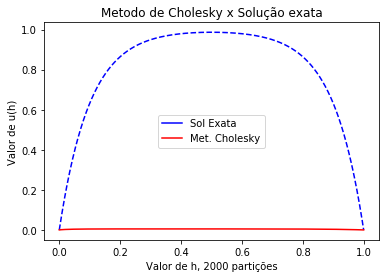
\includegraphics [width=5cm,height=5cm]{Cho2000part.png}
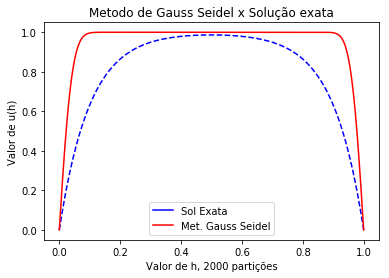
\includegraphics [width=5cm,height=5cm]{GS2000part.png}
\end{figure}

\newpage
\exec Seja o sistema linear:
$$
\mathbf{A}\mathbf{x}=\mathbf{b}
$$
onde,
$$
\mathbf{A} = A_{i,j} = \dfrac{1}{i+j+1} \quad \mbox{e} \quad \mathbf{b}=b_i =\dfrac{1}{i+n+1} .
$$
Supondo a matriz $\mathbf{A}_{n\times n}$, com diferentes dimensões $n$ (ex. $n = 10, 100, 1000$),  faça:

\begin{itemize}
\item Resolva utilizando o método de eliminação de Gauss \textbf{sem} e \textbf{com} pivoteamento e a decomposição LU.

\item Determine o erro cometido, por cada um dos métodos utilizados, através do resíduo calculado na norma do máximo, dado por:
$$
\|\mathbf{A}\mathbf{x} - \mathbf{b}\|_{\infty} = \max_{1\leq i\leq n}|A_{i,j}x_{i} - b_{i}|, \quad \forall j \in [1,n]
$$
onde $x_{i}$ é o vetor solução. Compare e discuta os resultados.

\end{itemize}


\end{itemize}

\text Supondo matrizes de dimensões 10,100 e 1000; Para 10 elementos:

\begin{table}[h]
\centering
  \begin{tabular}{l||l|l|l}
     & $ Gauss$ & $Gauss$ $com$ $Pivoteamento$ $Parcial$ & $LU$ \\
    \hline
    
    PASSOS & 375 & 475 & 440 \\
    
    TEMPO DE EXECUÇÃO & 0:00:00.000989 & 0:00:00.000997 & 0:00:00.000990 \\
    
    \hline
  \end{tabular}
  \caption{Comparação de resultados de diferentes dimensões}
\end{table}

\begin{table}[h]
\centering
  \begin{tabular}{l||l|l|l}
     & $ Gauss$ & $Gauss$ $com$ $Pivoteamento$ $Parcial$ & $LU$ \\
    \hline
    
    Erro Max & 27717.293488028645 & 2.7755575615628914e-16 & 2.0816681711721685e-16 \\
    
    
    \hline
  \end{tabular}
  \caption{Comparação de erros}
\end{table}

\begin{figure}[!htb]
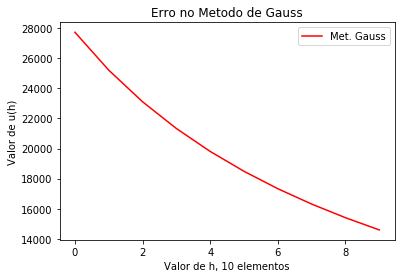
\includegraphics[width=7cm,height=5cm]{EGauss10part.png}
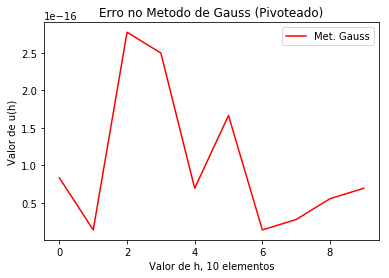
\includegraphics [width=7cm,height=5cm]{EGaussP10part.png}
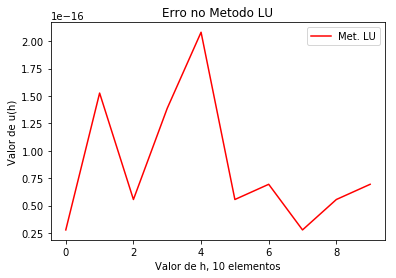
\includegraphics [width=7cm,height=5cm]{ELU10part.png}
\end{figure}



\newpage


Para 100:
\begin{table}[h]
\centering
  \begin{tabular}{l||l|l|l}
     & $ Gauss$ & $Gauss$ $com$ $Pivoteamento$ $Parcial$ & $LU$ \\
    \hline
    
    PASSOS & 338250 & 348250 & 343400 \\
    
    TEMPO DE EXECUÇÃO &  0:00:00.156041 & 0:00:00.100983 & 0:00:00.085986 \\
    
    \hline
  \end{tabular}
  \caption{Comparação de resultados de diferentes dimensões}
\end{table}

\begin{table}[h]
\centering
  \begin{tabular}{l||l|l|l}
     & $ Gauss$ & $Gauss$ $com$ $Pivoteamento$ $Parcial$ & $LU$ \\
    \hline
    
    Erro Max & 59153715.99267997 & 3.9898639947466563e-17 & 3.452099717193846e-16 \\
    
    
    \hline
  \end{tabular}
  \caption{Comparação de erros}
\end{table}

\begin{figure}[!htb]
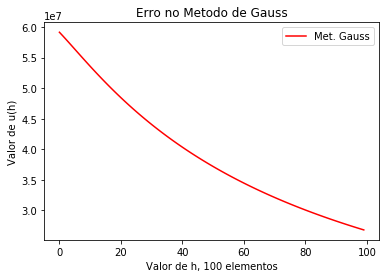
\includegraphics[width=7cm,height=5cm]{EGauss100part.png}
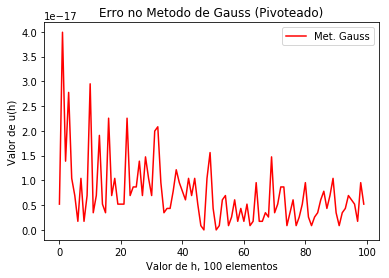
\includegraphics [width=7cm,height=5cm]{EGaussP100part.png}
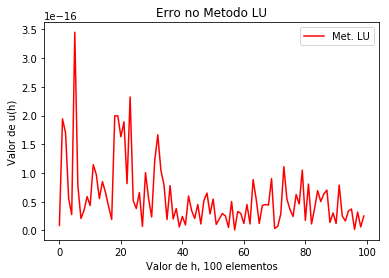
\includegraphics [width=7cm,height=5cm]{ELU100part.png}
\end{figure}

\newpage
Para 1000 elementos:

\begin{table}[h]
\centering
  \begin{tabular}{l||l|l|l}
     & $ Gauss$ & $Gauss$ $com$ $Pivoteamento$ $Parcial$ & $LU$ \\
    \hline
    
    PASSOS & 333832500 & 334832500 & 334334000\\
    
    TEMPO DE EXECUÇÃO &  0:01:38.251980 & 0:01:40.540858 & 0:05:04.649882\\
    
    \hline
  \end{tabular}
  \caption{Comparação de resultados de diferentes dimensões}
\end{table}

\begin{table}[h]
\centering
  \begin{tabular}{l||l|l|l}
     & $ Gauss$ & $Gauss$ $com$ $Pivoteamento$ $Parcial$ & $LU$ \\
    \hline
    
    Erro Max & 140669356.34659576 & 1.9081958235744878e-17 & 3.3881317890172013563e-20\\
    
    
    \hline
  \end{tabular}
  \caption{Comparação de erros}
\end{table}

\begin{figure}[!htb]
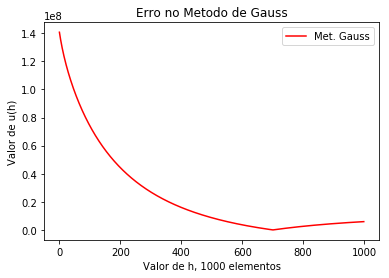
\includegraphics[width=7cm,height=5cm]{EGauss1000part.png}
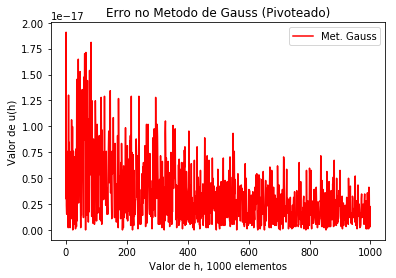
\includegraphics [width=7cm,height=5cm]{EGaussP1000part.png}
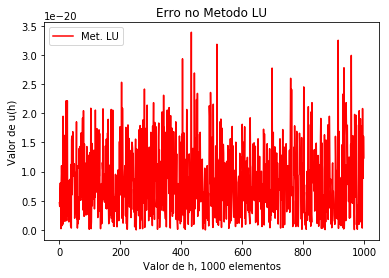
\includegraphics [width=7cm,height=5cm]{ELU1000part.png}
\end{figure}


\end{document}
